\chapter{Discussion} \label{Discussion}
\lhead{Chapter 5. \emph{Discussion}} 
%----------------------------------------------------------------------------------------

\section{The Future of Dynamic long RNAs}

  Deep sequencing of transcriptomes has revolutionized biology. Previously, transcript discovery was a cumbersome task. Transcript identification and characterization involved significant labor, cost, and materials. In the mid-90's, microarray technology \citep{Schena1995a} gave us a tantalizing glimpse into how genes were expressed, but were limited to probed, and therefore known, sequences. Yet, the green and red landscapes of a microarray analysis hinted at incredible complexity \textemdash a complexity that would have to wait for technology to catch up.

  Like many transformative technologies, RNA-seq was made possible by incremental improvements to numerous supportive technologies such as: 1) digital optics; 2) microscopy; 3) slide chemistry and on-slide PCR; and 4) nucleic-acid alignment. A HiSeq 2500 relies on all of these technologies (and others) to produce the 100M+ sequences that allow scientists to peer every day into the transcriptional output of a genome.

  In the past 5 years, biologists have started to think way beyond mRNAs and small RNAs. The former captured out interest for 30+ years \citep{Furuichi1975,Wei1975}, and the later has been on a run-away train since capturing out attention in 1998 \citep{Fire1998}. HTS has added long RNAs to these classes of gene products. However, many biologically-trained and minded Scientists find themselves overwhelmed by the complete different methods and approaches to tackling the ``big data'' created by modern genome-wide experiments. Experimental training does not currently provide students with the required skills in statistics, computer programing, and experimental design that are needed to work with genome-wide data (see section \ref{subsec: Biologists need Comp Skills}. The richness of this data often leaves many unasked (and unanswered) test-able hypothesis just sitting in public repositories \citep{Plocik2013}.

  At this point, it is important to remember that in this document \textit{long RNAs} may also refer to products containing characteristics of traditional mRNAs, that is a 5\textprime~m7G Cap, ligated exons, and a Poly(A) tail. However, many of these long mRNAs are extremely dynamic. So much so that until HTS and RNA-Seq, comprehensive investigation of their complexity was not possible.

  \subsection{Pervasive transcription}

    The encode project revealed that most of the genome is transcribed into RNA. This was done in cancerous cell lines, and while it revealed the potential for transcription, it did not reveal much biology beyond cells in culture simply perpetuating their existence. 

    \todo[line]{ Insert ENCODE References and Graur References} 
    The ENCODE papers from late 2012 suggested that 95\% of the genome is functional ($REF$). \citet{Djebali2012} focused on issues of transcription in these cell lines, as discussed in section \ref{sec:IsoformsPerGene}. The ENCODE studies were performed an human cancerous cell lines from different sources, and they still saw tremendous transcriptional diversity. Will better HTS tools and resolution, we should fully expect ever more diversity from the transcriptome once we can accurate catalogue and assemble transcripts from tissues, cells, and single single cells \textit{over time}.

  \subsection{Accurate and complete transcript annotation}

    A deck of cards has only 52 cards, but can delt into $2,598,960$ different 5 cards hands, as when playing Poker. There are $1,098,240$ different single-pair combinations, with a probability of obtaining one being almost 50\%. Compare this to ``Royal Flush'', for which there are only 4 options, and a probability of $649,739:1 or 1.54 * 10^{-6}$ !. It is these numbers that makes possible to play Poker for hours on end. Long ago, biologic evolved to arrange genes into unique and rare combinations, especially in eukaryotic organisms. Indeed the process of splicing is closely correlated with organism complexity. The process of AS is even more closely tied to organism complexity (see figure \ref{fig:numGenesAndNumSpliced}).

    Accurate determination and assembly of each card (exon) that comprises a hand (transcript) is a major known unknown of research into long RNA. The current state of the field is described in section \ref{subsec: Tx Assembly}. This field is in its infancy. Each gain in resolution or sensitivity reveals more complexity. Yet transcript assembly algorithms only provide predictions and probabilities for the existence of real molecules. Until RNA can be directly sequenced, in their entirety, from single cells, researchers will always be making compromises for transcript annotation and quantification. Once technology advances to the point where a transcriptome can be as accurately and quickly determined as a genome, extremely exiting research into the more subtle and nuanced complexity (e.g. what makes one twin molecularly different from another?) of biology can be unlocked.

    \todo[inline]{What is required to better transcript annotation?} % **************************

  \subsection{Tissue and cell specificity}

    \todo[inline]{Your feelings on tissue Specificity of long RNA expression} % **************************

\section{Lingering Questions for \dscam{}}

  What controls the stochastic and probabilistic splicing of \dscam{}? Why is it different between hemocytes and neurons? Why would hemocytes need less apparent diversity, given the range of antigen they could potentially encounter?

\section{In the haystack: piRNA precursor transcripts surrounded by RNA}


  Chapter \ref{MolCel} describes efforts to annotate XX transcripts from XX loci that account for XX\% of the total piRNAs in 14.5 dpp mice. 
  \todo[fancyline]{Insert these values} % **************************
  Also descibed is how these transcripts are typical Pol II transcripts, possesing all the archetypical molecular signatures including 5\textprime~MeGppp caps, introns, and poly(A) tails. Yet RNA from these molecules appears to be rapidly consumed and processed into millions of unique 24\textendash32 nt species. How does the cell partition long RNAs for translation by the ribosome (as the case for most mRNAs) or cleavage and maturation into piRNAs? The sections below propose experiments aimed toward answering this question.

  \subsection{How are they generated?}

    % From the resources paper: Indeed, two isoforms of pi-Wdfy3 are transcribed from different promoters in the testis (Figure S2D). The short isoform is transcribed from a low CpG promoter bound by A-MYB, while the long isoform is transcribed from a high CpG with no detectable A-MYB binding. piRNAs derive from the genomic region corresponding to the short transcript. In an A-Myb mutant, piRNA from the pi-Wdfy3 loci are reduced 165-fold (31.6 rpkm in heterozygotes versus 0.191 in mutants). The abundance of long isoform transcripts did not decrease (2.08 rpkm in heterozygotes versus 3.86 rpkm in mutant), while the small isoforms became undetectable (10.0 rpkm versus 0 rpkm), consistent with the idea that the short, but not the long, Wdfy3 transcript is a piRNA precursor RNA. Little is known about the regulation of genic piRNAs, because only seven genic piRNA loci are A-MYB-dependent (Li, et al., accompanying manuscript). We do not yet know if such differential regulation of transcript isoforms occurs more generally for genic piRNA loci.

    %How does cell partition prepachytene transcripts to mRNA or piRNA use?
    What determines that a seemingly mRNA-like piRNA precursor is processed into piRNAs, and not translated like crazy by Ribosomes?  Everything meets the ribosome ($REF$), so why is it that precursors are given a different lot in life?

    \begin{figure}[htbp] % pi-Wdfy3 expresses both mRNA and piRNA precursor transcript
      \centering 
      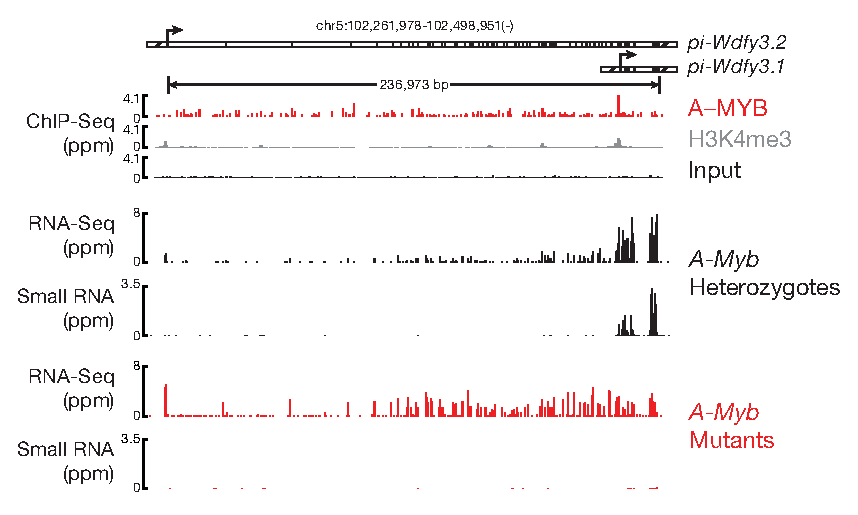
\includegraphics{Figures/Discussion/pi-wdfy3.eps}
      \caption[\wdfy{} locus expresses both mRNA and piRNA precusor form in testes]
      {\wdfy{} locus expresses both mRNA and piRNA precusor form in testes\\
        The mouse genomic locus \wdfy{} expresses both a traditional mRNA form, originating from an upstream TSS, and a piRNA precursor transcript from a downstream TSS. The piRNA precursor form appears to originate from an A-MYB-bound promoter, and is expressed in \amyb{} heterzygous mice. Also smalll RNAs (piRNAs) mapping to this locus are only observed in \amyb{} heterzygous mice, and not in \amyb{} mutant mice.
        }
      \label{fig:wdfy3}
      \end{figure}

    %Interaction w/ ribosomes?

  \subsection{What are they doing?}

    \todo[inline]{What are piRNAs doing in Mammals?} % **************************

  \subsection{In vivo chemical labeling of precursor piRNA transcripts}

    % From Resources Paper: Despite sharing many features with protein-coding genes, intergenic piRNA loci stand out as a unique class of transcriptional units. Almost half contain no introns

    % Need section here on the chemical modification - what were you thinking? Azide? Par-Clip?  Maybe a CLASH-like assay?  What about what Mihir is developing?
    
    SeqZip accurately reports on the presence of multiple, distant sequences contained in the same RNA molecule (see Chapters \ref{Chapter2} and \ref{Chapter3}). Yet I was not able to observe ligation products templated off some of the most highly-expressed precursor transcripts (see section \ref{sec: precursor TX}. We hypothesize that the most likely explanation for being unable to observe ligation products for these transcripts, but successfully observing those for a very long, but lowly expressed gene   extit{Dst}, suggests that precursor transcripts are rapidly processed into mature piRNAs. What if this is not the case if we could hybridize ligamers to precursor transcripts in vivo? Put another way  extemdash What if the steady-state amount of precursor transcript is very low due to rapid processing, but when visualized in real time, the transcripts are of sufficient abundance for FISH? Ligamers could be engineered to contain different combinations of fluorescent dyes, and the proximity and intensity of the signal could be used to infer precursor transcripts. Importantly, this approach could distinguish long, continuous precursor transcripts from processing intermediates and mature piRNAs.

  \subsection{In vivo imaging of precursor piRNA transcripts}

    %Another idea would be to image the precursors in real time somehow. How about tagging them and following them in the sperm? That could be cool. You could even follow them into the developing embryo. 
    The most important question for mammalian \textit{pachytene} piRNAs is \textit{What are they doing?}. We know that they are essential for the health of the species, as discussed in section \ref{c3-intro}, and piRNA-pathway mutants are sterile. What could these small RNAs, with complementarity to nothing but themselves, be doing? Building on the last section discussing chemical modification precursor transcripts, if the modification was again durable enough for downstream analysis, perhaps the modification would remain in the mature piRNAs that are incorporated into mature sperm. These modifications could be tracked as the sperm move through the \hl{semineferous tubues} and into the $SPERM ANATOMY$. One could even track the piRNAs as they fuse with the oocyte to create an embryo. If this modification was labile, piRNA interacting proteins or nucleic acids could be captured or marked as well, providing additional clues as to the function of piRNAs in sperm and early embryogenesis.

    The cellular location of precursor piRNA transcript processing is not known. The most accepted hypothesis is that precursor transcripts are processed into mature piRNAs with machinery tethered to chromatoid bodies ($REF$) or another structure similar to Drosophila Nuage ($REF$) near the mitochondrial cement ($REF$). Knowledge of \textit{where} mature piRNAs are generated would provide clues into larger mechanist details of their biogenesis. \todo[prepend]{Need Chromatoid References}

    I can think of two broadly different ways in which we could pinpoint the physical location of mature piRNA generation. The first is to chemically label, in some manner, primary piRNA transcripts. The label would need to 1) not interfere with processing and 2) be durable to later methods used to analyze the presence or absence of the modification. A second way to identify the location of mature piRNA processing would be to actually observe, through in vivo \hyperref[hd:abrevs]{FISH}, the various products and by-products of biogenesis. In this particular approach, SeqZip maybe useful.

    % MS2 lopp introduction into piRNA precursor transcripts.
    Another idea here would be to use the MCP x MBS mouse as published by the Singer lab \citep{Park2014}. In this paper they insert multiple MS2 binding loops into the 3  extprime~-UTR of the $beta$-actin gene, and cross it with another mouse that has MCP (MS2 Bacteriophage capsid protein) fused to GFP. Using this system they can visualize   \textit{endogenous} mRNAs in cultured MEF cells, and brain sections. How could we apply this to imaging of piRNA precursor transcripts? If we inserted an MS2 loop into the tail end of transcripts, what would we see? It is certainly worth it!

\section{Future uses of SeqZip}

  SeqZip can be used to many different forms of RNA sequence characterization. An incomplete illustration of these applications is shown in Figure \ref{fig: Panel of SeqZip Applications}. The three novel applications are discussed below:

  \begin{figure}[htbp] % SeqZip uses Panel
    \centering 
    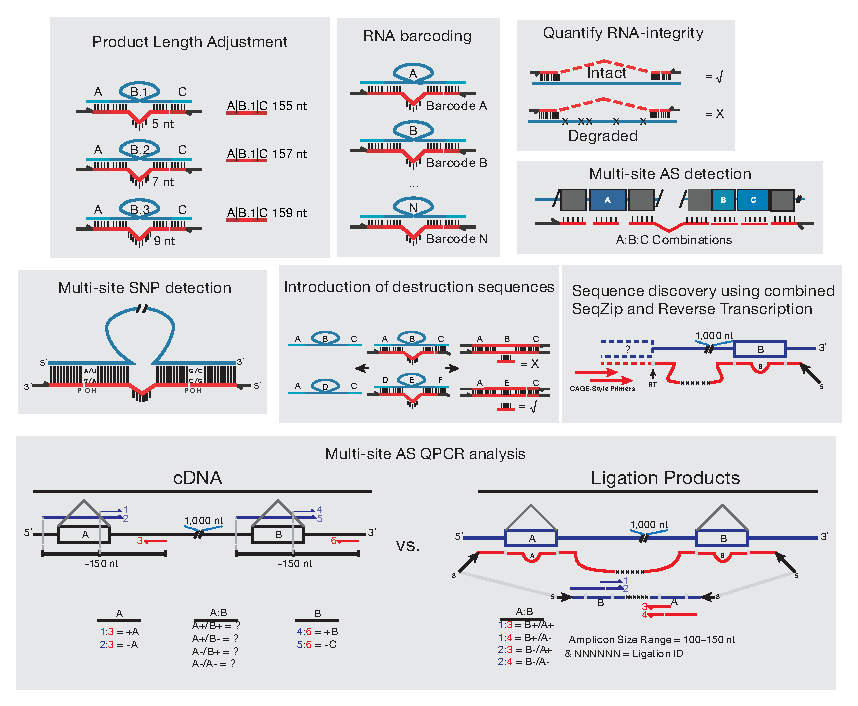
\includegraphics{Figures/Discussion/SeqZipUses.eps}
    \caption[Proposed uses of the SeqZip methodology]
    {Proposed uses of the SeqZip methodology \\
      Shown here are general applications of the SeqZip method to profiling RNA sequences. Top row examples are substantiated by experiements described on Chapters \ref{SeqZipPaper} and \ref{SeqZipMethod}, the middle and lower rows are hypothetical but logical extensions of the method.
      }
    \label{fig: Panel of SeqZip Applications}
    \end{figure}

  \subsection{Multi-site SNP detection}

    \todo[inline]{Mention Which side to put the Mismatch} % **************************
    % Cite the newest Shuman paper, and the Shuman crystal papers

  \subsection{Introduction of destruction sequences}

    \todo[inline]{Discuss Type III restriction enzymes, etc} % **************************

  \subsection{Multi-site SNP probes}

    % What about applying the Church lab's new technique of in situ sequencing? Would this help us differentiate transcripts from mature piRNAs?  

\section{SeqZip Assay Improvements}

  The SeqZip methodology as developed and described in Chapters \ref{SeqZipPaper} and \ref{SeqZipMethod} works adequately and robustly for characterization of relatively simple (\cd{}) to extremely complex (\dscam{}) genes. However, there is still substantial room for method optimization. Two obvious areas of improvement include the reduction of ligation time and NTL product formation. The improvements and modifications discussed below should assist in achieving these two (among other) goals.

  \subsection{LNA-containing ligamers and T39A Rnl2} 

    The use of an RNA-base on the 5\textprime~ side of the nick encourages a C3\textprime~\textit{endo} sugar pucker for the base, placing the 3\textprime~OH in an apical orientation relative to the the AMP leaving group (see Figure \ref{fig:Rnl2 and suger pucker}) \citep{Nandakumar2006}.

    \begin{figure}[htbp] % Rnl2 Suger Pucker
      \centering 
      \includegraphics{Figures/Discussion/Rnl2_and_suger_pucker.eps}
      \caption[Suger pucker in Rnl2 structures]
      {Suger pucker in Rnl2 structures \\
        Using two different nucleic acid substrate combinations crystallized with Rnl2, \citet{Nandakumar2006} demonstrates the effect of 3\textprime~ and 2\textprime~ identify of the base at the 5\textprime~ side of the nick: Left) The crystal structure (PDB: 2HVS), containing a 2\textprime~ position deoxy residue, displays a DNA-like C2\textprime~\textit{endo} sugar pucker. In contrast to Right) where the crystal structure (2HVR) contains a 2\textprime~ hydroxyl and displays an RNA-like C3\textprime~\textit{endo} sugar pucker.
        }
        \label{fig:Rnl2 and suger pucker}
        \end{figure}

    With lowered costs of oligo synthesis, incorporation of 2\textprime~OMe at the penultimate and ultimate bases of the 5\textprime~ nick ligamers should greatly increase ligaiton efficiency, as these are the primary substrate-specificity determinants of Rnl2 \citep{Nandakumar2004a, Nandakumar2006}.

    Interestingly, \citet{Nandakumar2004a} demonstrated that the ribosome at the penultimate position, evidenced by a 50-fold reduction in turnover number for 2\textprime~H substitutions at this position, compared to full activity for 2\textprime~OMe. \citet{Nandakumar2006} (see Figure \ref{fig:Rnl2 and suger pucker} shows that Threonine 39 (T39) hydrogen bonds with both the 2\textprime~OMe and 3\textprime~O of the penultimate suger. A T39A mutation did not phenocopy the 2\textprime~H substitution on the penultimate suger, indicating that suger pucker is the structural constraint on ligation efficiency. These results indicate that a T39A mutant of Rnl2 may demonstrate increased RNA-templated DNA:DNA ligation efficiency, as it would have one less molecular requirement for RNA.

    Future versions of the SeqZip assay could use a combination of LNA modified bases \citep{You2006} at either the penultimate or terminal residues on the 5\textprime~side of the nick in order to increase 1) specificity, and 2) enzyme efficiency. The combination of these modifications in the ligamers could be combined with a T39A mutant form of Rnl2 for a potentially greatly enhanced ligation rate.

  \subsubsection{Thermostable Ligases}

    The use of LNA-containing brings up issues involving off-target hybridization. Future iterations of the SeqZip methodology could use directed protein evolution of Rnl2 \citep{Stemmer1994, Romero2009a} to develop a thermostable variant of Rnl2, similar to variations of DNA ligase that have been used for years \citep{Barany1991}. Use of LNAs and elevated ligation temperatures could alviate off-target hybridization events reducing both nonproductive hybridization and non-templated ligation events. This would also allow for use of reduced overall ligamer concentrations, in line with the optimal SeqZip experiment described in section \ref{subsec: Ideal multiplex study} and synthesis on microarrays.

  \subsection{Re-purposing the SOLiD Platform}

    \todo[inline]{SOLiD Application of SeqZip} % **************************

    The ability to incorporate custom sequuences into ligations, which subsequently are incorporated into ligation products provides tremendous opportunities for downstream analysis (see figure \ref{fig: Panel of SeqZip Applications}).

  \subsection{Quantifying ligation and PCR events}

    Digital PCR of the PCR products ala \citep{Shiroguchi2012a}. 

  \subsection{Reducing required input RNA and ligamer concentration}

    SeqZip on single-cell RNA samples.

  \subsection{An ideal SeqZip experiment to query coordinated splicing}
    \label{subsec: Ideal multiplex study}

    If I could go back in time 4 years and still possess the knowledge and abilities that I do now, I would have approached a genome-wide study of coordination in splicing using SeqZip much differently. First, I would have focused on alternative first exon (or promoter, or TSS) and potential coordination with downstream cassette exons. I would have mined newly-generated RNA-Seq data \citep{Wang2008, Pan2008} for alternative first exons and cassette exons of sufficient expression. Then, I would have used my automated ligamer design software (see Appendix \ref{AppendixC}), to create a database of the required ligamers. As this would require at least 3 ligamers per event, with very little duplicated use of ligamers, the number of ligamers would make standard synthesis, even using 384-well plates, impossible. Therefore, I would have pursued printing the ligamers on a custom microarray, and cleaved them into solution, similar to products offered by \href{http://www.nimblegen.com/}{Nimblogen{. These ligamers would be barcoded and priming sequences included such that short (50nt) paired-end reads could reliably identify the templating first and cassette exons. Using this pool of ligamers, I would have performed the SeqZip assay, including a barcoding scheme to quantify the number of ligation events per {alt first exon::cassette exon} pair. Also, the libraries would have been amplified via digital PCR allowing me to check for PCR jackpots \citep{Shiroguchi2012a}. Finally, the data would be aligned against a reference of all {alt first exon::cassette exon} pairs, and any potential coordination determined.

    If I could have done the experiment designed above, I feel the full potential and utility of the SeqZip method could have been realized and generated new and valuable knowledge for the field of gene expression.

  \subsection{SeqZip and single-molecule FISH}

    \begin{figure}[htbp] % Multi-site Fish using SeqZip
      \centering 
      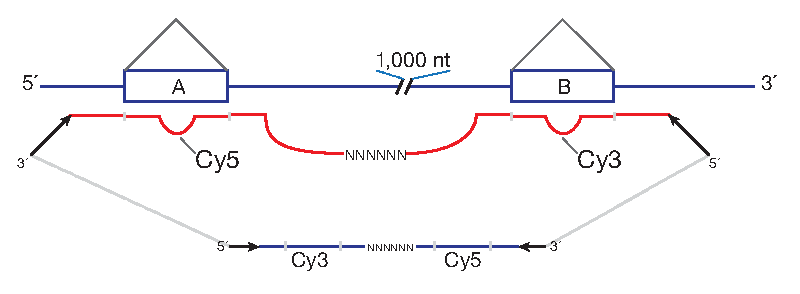
\includegraphics{Figures/Discussion/MultiSiteFish.eps}
      \caption[Multi-Site smFISH using flourophore-containg ligamers]
      {Multi-Site smFISH using flourophore-containg ligamers \\
        \hl{Insert Caption Here}
        }
      \label{fig:MultiSite FISH using SeqZip}
      \end{figure}

\section{Final thoughts}

  \subsection{Biologists need Computation Biological Skills}\label{subsec: Biologists need Comp Skills}

    Just 10 years ago,  Graduate students and PhDs in the fields of Molecular Biology or Biochemistry need not venture far from data analysis within Excel or perhaps a statistical program with an advanced graphical interface (examples include Prism or Graphpad). Software knowledge that stops at these tools and the rest of the Microsoft Office suite of tools is no longer enough to generate big strides in Biomedical research.

    Working with tens of even hundreds of lines of data within a spreadsheet is manageable and computers from 20 years ago had more then enough computing power to process the data. Yet, this type of data is longer then endpoint of most cutting edge projects. Many students and post docs often find that they are unable to analyze the data generated from months or years of tireless bench work. Faced with learning what is effectively a collection of new languages and awash in a sea of acronyms (LINUX, BASH, GNU, PERL, R) they reach out for help from a ``Bioinformatics person.'' Perhaps the relationship and interaction with this personal is productive, leading to a collaboration and exciting new knowledge. Sometimes it isn't, and the bench scientist shifts into one of three modes: 1) Wait; 2) Find another bioinformatic-minded collaborator; or 3) collect more data.

    In my experience, the most often chosen mode is ``wait.'' This is also the most damaging, as it delays the progress of one's work, and the advancement of science in general. Personally, I did not want to fall into this mode, and once the multiplex study described in section \ref{sec: Multiplex Gene Study} reached a point where I had millions of sequencing reads, but I could not find anyone to help me analyze the data, that I decided to educate myself on the basic principles of Linux, the command line, and analysis of HTS data.

    A Biologically-train individual who posses the knowledge of analysis of HTS datasets is an extremely powerful and empowering situation. This was recently commucated in \citet{Plocik2013}:

    \begin{quote} % Polick2013 Quote about insight without a Pipette
      \itshape 
      Such exercises will empower students to explore and assess the quantitative data published in the manuscripts that they read, which can no longer be assessed at a glance like the qualitative gel-based results on which molecular biology was founded. Ultimately, it will be equally important to know how to write code as it is to pipette. - \citep{Plocik2013}
      \singlespacing
      \end{quote}

    The fact is that no one will care about a project as much as the Graduate student or PostDoc who is the main project driver. Learning and training of computational skills bent on analyzing large datasets should be central to the education in Biomedical sciences in the future.

  \subsection{Science versus Engineering: Two thoughts in one school}

    \begin{quote}
      \itshape 
      \singlespacing
        “There is a general attitude among the scientific community that science is superior to engineering.” - \citep{Macilwain2010}

      “Science is about what is; engineering is about what can be. Engineers are dedicated to solving problems and creating new, useful, and efficient things.“ - Niel Armstrong
      \end{quote}

    A common schism between technically-oriented individuals is whether or not they identify themselves as an engineer or a scientist. The first quote, from an article published in Nature, communicates a clear bias in academic circles of the importance of the   extit{why} over the   extit{how}. In essence, how one priorities these questions may categories individuals as a scientists (why is important) or an engineer (how is more important). The second quote, from the first man to walk on the Moon, Neil Armstrong, highlights what motivates a self described ”engineer” and ”geek.” How does a single graduate system, training PhDs for careers in life science, educate individuals who fall into these two fundamentally different belief systems?
    In short  extemdash not well. When searching for a lab to call home, I told professors that I wanted to work on a technology development project. A typical response was, “That's not what we do here.” As someone who is first interested in the ``how'' over the ``why,'' this began a brief period when I thought I had made the wrong choice in leaving industry to go back to graduate school. What was the basis for this aversion to technology development? The same article in Nature states that this feeling toward engineering may be attributed:

    \begin{quote} 
      \itshape 
      \singlespacing
      ...partly to a ``linear'' model of innovation, which holds that scientific discovery leads to technology, which in turn leads to human betterment.  This model is as firmly entrenched in policy-makers' minds as it is intellectually discredited.  As any engineer will tell you, innovations, such as aviation and the steam engine, commonly precede scientific understanding of how things work.
      \end{quote} 

    If policy-makers value basic discovery over technological application, perhaps this explains why many of my professors tried to steer me away from a technology development project.

    In spite of policy-makers and my professors holding the viewpoint that discovery precedes technology, some of the most notable breakthrough scientific discoveries, including many made by Nobel Laureates, demonstrate a clear integration of both the scientific method and technological application.  For example, the 2007 award in Physiology and Medicine was given for “discoveries of principles for introducing specific gene modifications in mice by the use of embryonic stem cells."  By combining these principle discoveries, an indispensable technique in modern genetics was created – gene targeting.  The feeling of which is more important, the principle discoveries or the application thereof, is likely what separates a scientist from an engineer. 

    The importance of technology to the advancement of science in general is not limited to anecdotes resulting in a Nobel prize. A quick scan of the most \href{http://www.pnas.org/reports/most-cited}{highly-cited} papers in the journal PNAS reveals that the top 13, indeed   extit{all} 13, are about a novel methodology or technique. Sequencing of DNA, microarray analysis, tetracycline-ineducable promoters, recombinant adenovirus, and site-specific mutagenesis are just a handful of the tools on this list. This effect can be seen in \href{http://simplystatistics.org/2014/04/07/writing-good-software-can-have-more-impact-than-publishing-in-high-impact-journals-for-genomic-statisticians/}{computation biology}, with transformative techniques, such as BLAT \citep{Altschul1990} and Bowtie \citep{Langmead2009} attaining citations well beyond a typical paper in their journal of publication and far more than most primary research-centered articles.

    How does someone who is motivated by the engineering of science best contribute in an academic setting? Luckily, I did not have to question my decision to return to school for long. I found a pair of labs where I could learn how to practice traditional hypothesis-driven research while also developing new tools necessary to do so. My project is a perfect fit for me and has been terrific fun to work on. In the past five years, the technique that I developed, SeqZip, allows for the more efficient study of  mRNA isoforms produced from alternative splicing of pre-mRNA. This is a very engineering-type accomplishment. However, the technique uses short DNA oligonucleotides and a novel activity (that I discovered) of an known RNA ligase to shorten and simplify isoform sequence information. Use of Rnl2 to perform RNA-templated DNA:DNA ligation is completely new knowledge, and falls squarely within a scientific purview. The technique simplifies many of the experimental issues that researchers struggle with when studying the often complex products of alternative splicing.
    
    \todo[inline]{Need transition or concluding paragraph} % **************************
    
  \subsection{Dealing with the data deluge}

    \todo[inline]{Writing about HTS data management}

    How do we work with all this data? Mention LabKey, GenomeBridge, Define the scope of the problem, etc...

    I would love to have a database of complete transcripts of a cell - think about how you were panning the data for the MolCel paper, and you could see ChIP marks, Pol II occupancy, RNA-Seq, and piRNA data. It would be great to be able to do that more often, and we greater precision
